\begin{figure*}[t]
\centering
\definecolor{oBlueL}{HTML}{DEEBF7}\definecolor{oBlueD}{HTML}{2E75B6}\definecolor{oOrangeP}{HTML}{FDF2E9}\definecolor{oOrangeL}{HTML}{FBE5D6}\definecolor{oOrangeD}{HTML}{C55A11}\definecolor{oOrangeS}{HTML}{ED7D31}\definecolor{oGreenS}{HTML}{C5E0B4}\definecolor{oGreyP}{HTML}{F2F2F2}\definecolor{oGreyL}{HTML}{E7E6E6}\definecolor{oGreyM}{HTML}{BFBFBF}\definecolor{oGreyS}{HTML}{A6A6A6}\definecolor{oGreyK}{HTML}{7F7F7F}\definecolor{oGreyD}{HTML}{595959}
\begin{tikzpicture}[x=1mm, y=1mm, >={Stealth[length=1.4mm, width=1.3mm]}]
\useasboundingbox (0,0) rectangle (174.00,-77.00);
\draw[draw=oGreyK, line width=0.36pt, dash pattern=on 3.2pt off 2.2pt, rounded corners=5pt] (27.64,-30.00) rectangle (53.58,-72.00);
\draw[fill=oOrangeP, draw=oOrangeD, line width=0.8pt, dash pattern=on 3.2pt off 2.2pt, rounded corners=5pt] (59.22,-30.00) rectangle (124.81,-72.00);
\draw[draw=oGreyK, line width=0.36pt, dash pattern=on 3.2pt off 2.2pt, rounded corners=5pt] (130.45,-30.00) rectangle (154.39,-72.00);
\draw[->, line width=0.6pt, draw=black] (11.00,-9.40) -- (16.64,-9.40);
\draw[->, line width=0.6pt, draw=black] (41.64,-9.40) -- (47.29,-9.40);
\draw[->, line width=0.6pt, draw=black] (68.29,-9.40) -- (73.93,-9.40);
\draw[->, line width=0.6pt, draw=black] (99.93,-9.40) -- (160.00,-9.40);
\draw[->, line width=0.6pt, draw=black] (167.00,-14.06) -- (167.00,-18.20) -- (29.14,-18.20) -- (29.14,-14.06);
\draw[->, line width=0.6pt, draw=black] (22.00,-41.06) -- (30.11,-41.06);
\draw[->, line width=0.6pt, draw=oBlueD] (40.61,-45.71) -- (40.61,-48.89);
\draw[->, line width=0.6pt, draw=black] (51.11,-53.54) -- (56.40,-53.54) -- (56.40,-35.07) -- (61.69,-35.07);
\draw[->, line width=0.6pt, draw=oOrangeD] (75.19,-38.14) -- (75.19,-41.31);
\draw[->, line width=0.6pt, draw=oOrangeD] (75.19,-50.63) -- (75.19,-53.80);
\draw[->, line width=0.6pt, draw=oOrangeD] (88.69,-45.97) -- (94.34,-45.97);
\draw[->, line width=0.6pt, draw=black] (122.34,-41.00) -- (132.92,-41.00);
\draw[->, line width=0.6pt, draw=oGreyD] (142.42,-44.07) -- (142.42,-47.24);
\draw[->, line width=0.6pt, draw=black] (151.92,-51.90) -- (160.00,-51.90);
\draw[->, line width=0.6pt, draw=black] (167.00,-56.56) -- (167.00,-75.00) -- (11.00,-75.00) -- (11.00,-58.40);
\node[font=\rmfamily\fontsize{8.5}{10.20}\selectfont, text width=70.00mm, align=left, inner sep=0, anchor=west] at (0.00,-1.80) {\textbf{(a)\ EB prompt (benchmark agent)}};
\node[inner sep=0, anchor=north west] at (0.00,-3.90) {
\includegraphics[width=11.00mm, height=11.00mm]{fig/arch_ebframe.png}};
\draw[black, line width=0.19pt] (0.00,-3.90) rectangle (11.00,-14.90);
\filldraw[fill=oGreyL, draw=black, line width=0.36pt, rounded corners=2.6pt] (16.64,-4.74) rectangle (41.64,-14.06);
\node[font=\rmfamily\fontsize{7.5}{9.00}\selectfont, text width=20.06mm, align=center, inner sep=0, anchor=center] at (29.14,-9.40) {instruction $\ell$,\\examples, log $h_t$};
\filldraw[fill=oBlueL, draw=black, line width=0.36pt, rounded corners=2.6pt] (47.29,-4.74) rectangle (68.29,-14.06);
\node[font=\rmfamily\fontsize{7.5}{9.00}\selectfont, text width=16.06mm, align=center, inner sep=0, anchor=center] at (57.79,-9.40) {VLM $f$\\[-0.2mm]{\fontsize{6.5}{7}\selectfont\itshape frozen}};
\filldraw[fill=oGreyL, draw=black, line width=0.36pt, rounded corners=2.6pt] (73.93,-4.74) rectangle (99.93,-14.06);
\node[font=\rmfamily\fontsize{7.5}{9.00}\selectfont, text width=21.06mm, align=center, inner sep=0, anchor=center] at (86.93,-9.40) {text plan of\\action ids};
\filldraw[fill=oGreenS, draw=black, line width=0.36pt, rounded corners=2.6pt] (160.00,-4.74) rectangle (174.00,-14.06);
\node[font=\rmfamily\fontsize{7.5}{9.00}\selectfont, text width=9.06mm, align=center, inner sep=0, anchor=center] at (167.00,-9.40) {actions\\$u_{t:t+m}$};
\node[font=\rmfamily\fontsize{6.5}{7.80}\selectfont\itshape, text width=52.07mm, align=center, inner sep=0, anchor=center] at (129.97,-6.70) {spatial state only in generated text};
\fill[white] (118.00,-16.95) rectangle (134.00,-19.45);
\node[font=\rmfamily\fontsize{7.0}{8.40}\selectfont, text width=16.00mm, align=center, inner sep=0, anchor=center] at (126.00,-18.20) {feedback};
\node[font=\rmfamily\fontsize{8.5}{10.20}\selectfont, text width=70.00mm, align=left, inner sep=0, anchor=west] at (0.00,-22.80) {\textbf{(b)\ \ours (ours)}};
\node[font=\rmfamily\fontsize{8.5}{10.20}\selectfont\bfseries\itshape, text width=25.34mm, align=left, inner sep=0, anchor=west] at (28.24,-27.60) {Per-image questions};
\node[font=\rmfamily\fontsize{8.5}{10.20}\selectfont\bfseries\itshape, text width=64.98mm, align=left, inner sep=0, anchor=west] at (59.82,-27.60) {Metric hypothesis memory};
\node[font=\rmfamily\fontsize{8.5}{10.20}\selectfont\bfseries\itshape, text width=27.94mm, align=left, inner sep=0, anchor=west] at (131.05,-27.60) {Search and control};
\node[font=\rmfamily\fontsize{7.0}{8.40}\selectfont, text width=22.00mm, align=center, inner sep=0, anchor=center] at (11.00,-32.60) {frame $I_t$,\\phrase $s$};
\node[inner sep=0, anchor=north west] at (0.00,-36.40) {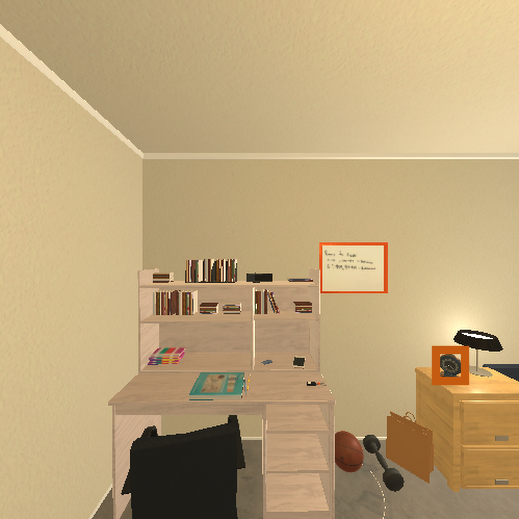
\includegraphics[width=22.00mm, height=22.00mm]{fig/arch_frame.png}};
\draw[black, line width=0.19pt] (0.00,-36.40) rectangle (22.00,-58.40);
\filldraw[fill=oBlueL, draw=black, line width=0.36pt, rounded corners=2.6pt] (30.11,-36.40) rectangle (51.11,-45.71);
\node[font=\rmfamily\fontsize{7.5}{9.00}\selectfont, text width=16.06mm, align=center, inner sep=0, anchor=center] at (40.61,-41.06) {VLM $f$\\[-0.2mm]{\fontsize{6.5}{7}\selectfont\itshape frozen}};
\filldraw[fill=oGreyP, draw=black, line width=0.36pt, rounded corners=2.6pt] (30.11,-48.89) rectangle (51.11,-58.20);
\node[font=\rmfamily\fontsize{7.5}{9.00}\selectfont, text width=16.06mm, align=center, inner sep=0, anchor=center] at (40.61,-53.54) {presence $\pi_t$\\box $b_t$};
\filldraw[fill=oOrangeL, draw=black, line width=0.36pt, rounded corners=2.6pt] (61.69,-32.00) rectangle (88.69,-38.14);
\node[font=\rmfamily\fontsize{7.5}{9.00}\selectfont, text width=22.06mm, align=center, inner sep=0, anchor=center] at (75.19,-35.07) {lift with $D_t$, $p_t$};
\filldraw[fill=oOrangeL, draw=black, line width=0.36pt, rounded corners=2.6pt] (61.69,-41.31) rectangle (88.69,-50.63);
\node[font=\rmfamily\fontsize{7.5}{9.00}\selectfont, text width=22.06mm, align=center, inner sep=0, anchor=center] at (75.19,-45.97) {fuse viewpoints,\\negative evidence};
\node[inner sep=0, anchor=north west] at (61.69,-53.80) {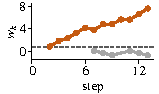
\includegraphics[width=27.00mm, height=16.20mm]{fig/arch_evidence.pdf}};
\node[inner sep=0, anchor=north west] at (94.34,-32.00) {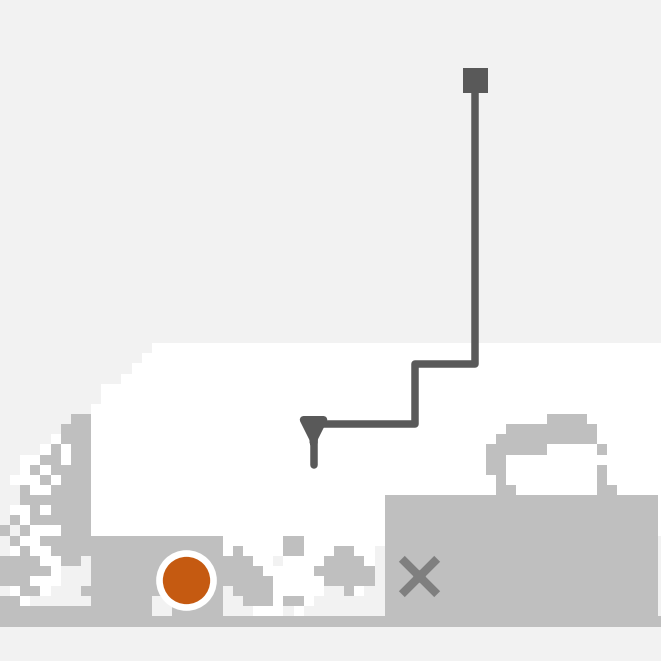
\includegraphics[width=28.00mm, height=28.00mm]{fig/arch_bev.png}};
\draw[black, line width=0.19pt] (94.34,-32.00) rectangle (122.34,-60.00);
\node[font=\rmfamily\fontsize{7.0}{8.40}\selectfont, text width=28.00mm, align=center, inner sep=0, anchor=center] at (108.34,-63.80) {hypotheses $\mu_k$\\on the map $M_t$};
\filldraw[fill=oOrangeL, draw=black, line width=0.36pt, rounded corners=2.6pt] (132.92,-37.93) rectangle (151.92,-44.07);
\node[font=\rmfamily\fontsize{7.5}{9.00}\selectfont, text width=14.06mm, align=center, inner sep=0, anchor=center] at (142.42,-41.00) {select $k^\star$};
\filldraw[fill=oGreyL, draw=black, line width=0.36pt, rounded corners=2.6pt] (132.92,-47.24) rectangle (151.92,-56.56);
\node[font=\rmfamily\fontsize{7.5}{9.00}\selectfont, text width=14.06mm, align=center, inner sep=0, anchor=center] at (142.42,-51.90) {A* planner\\on $M_t$};
\filldraw[fill=oGreenS, draw=black, line width=0.36pt, rounded corners=2.6pt] (160.00,-47.24) rectangle (174.00,-56.56);
\node[font=\rmfamily\fontsize{7.5}{9.00}\selectfont, text width=9.06mm, align=center, inner sep=0, anchor=center] at (167.00,-51.90) {action\\$u_t$};
\fill[white] (76.00,-73.75) rectangle (104.00,-76.25);
\node[font=\rmfamily\fontsize{7.0}{8.40}\selectfont, text width=28.00mm, align=center, inner sep=0, anchor=center] at (90.00,-75.00) {next frame};
\end{tikzpicture}
\caption{\textbf{(a)}~The EB prompt maps $I_t$, the instruction $\ell$, and the history $h_t$ to a text plan $u_{t:t+m}$ with the VLM $f$. \textbf{(b)}~\ours asks $f$ for the presence $\pi_t$ and box $b_t$ of the phrase $s$, lifts them with depth $D_t$ and pose $p_t$ into hypotheses $\mu_k$ with evidence $w_k$, selects $k^\star$, and plans $u_t$ on the map $M_t$. Thumbnails: a Long-horizon test episode; the target (orange) passes the commit threshold (dashed) and two look-alikes (grey) fall below zero.}
\label{fig:arch}
\end{figure*}
